%TODO: MarginPars zetten
\chapter{Onderzoek: SOUP analyse}\label{ch:onderzoek:-soup-analyse} % Chapter title
Bronnen:

\begin{itemize}
    \item https://medium.com/@manjula.aw/nodejs-security-tools-de0d0c937ec0
    \item
\end{itemize}
\begin{itemize}
    \item Javascript     https://github.com/RetireJS/retire.js
    \item SBT https://github.com/albuch/sbt-dependency-check
    \item
\end{itemize}
Dit hoofdstuk geeft het onderzoek weer naar een methode om gegevens over dependencies vanuit de bestaande pipeline in de module te krijgen. Waarbij rekening gehouden wordt met zowel het ontwerp en functionaliteit van de huidige pipeline en de informatie behoefte van de module. Om tot een resultaat te komen in dit onderzoek is de volgende onderzoeksvraag opgesteld: "Welke methoden zijn er om gegevens over depenendencies binnen bestaande projecten te verkrijgen, en wat zijn de implicaties die deze methoden mee brengen?" Uit deze onderzoekvraag komen de volgende deelvragen:
\begin{itemize}
    \item Welke tools bestaan er om dependency informatie uit een sbt en npm project te halen?
    \item Hoe zijn de tools in te zetten in de huidige projecten?
    \item Welke output wordt er verkregen van de tools?
    \item Welke manieren zijn er om uit de huidige pipeline informatie over de deploy te halen?
    \item Wat zijn hier de voor en nadelen van?
\end{itemize}
De deelvragen worden ieders in een eigen sectie beantwoord. Hierdoor is er voldoende informatie om een juiste conclussie te trekken
Door het beantwoorden van de vragen kan er een conclussie worden getrokken over de manier van het verkrijgen van de benodigde informatie de vervolgens door module verwerkt kan worden om op die manier inzichten in veilige software te verkrijgen.



\section{Welke tools bestaan er on dependency analyses uit te voeren op dev-stack van Eaglescience.}\label{sec:welke-tools-bestaan-er-on-dependency-analyses-uit-te-voeren-op-dev-stack-van-eaglescience.}
Zoals eerder onderzocht zijn er drie belangrijke onderdelen binnen de dev stack waarop gecontroleerd dient te worden: SBT voor Scala backend projecten en NPM voor de node.js 'frontend' projecten. Als we de dev\-stack systematisch van gebruiker naar platform aflopen is eerst NPM aan de beurt en vervolgens SBT. Zoals in het vorige onderzoek naar boven is gekomen heeft de OWASP als doel software veiliger te maken. Te lezen was dat ze dit deels doen door awareness middels de top-10 en symposia te houden. Echter zijn er ook proactievere projecten binnen OWASP, zoals de ontwikkeling van een dependency check. (https://owasp.org/www-project-dependency-check/). Deze dependency check is geschikt voor de meest voorkomende talen die gebruikt worden, echter is Scala niet veel gebruikt en wordt dus niet direct ondersteunt. Verder onderzoek binnen het project geeft weer dat het voor Node projecten wel ondersteuning bied middels de NPM -audit tool die al in NPM ingebouwd is op dependencies te scannen. Dit project lijkt dus niet voor de hand liggend om te gebruken. Maar bied wel mogelijkheden om als startpunt te gebruiken.

Binnen de OWASP bestaat er een werkgroep die zich bezig houden met het scannen van kwetbaarheden in dependencies: https://owasp.org/www-project-dependency-check/  De OWASP is als uitgangspunt genomen voor het zoeken naar tooling die gebruikt kan worden voor het analyseren van de projecten.


\subsection{NPM}\label{subsec:npm}
Als de OWASP Dependency check documentatie na wordt gelezen bestaat er geen directe module voor het checken van NPM packages. (https://jeremylong.github.io/DependencyCheck/analyzers/index.html). Er wordt zelfs aangegeven dat het gebruik maakt van een tool ingebouwd in NPM genaamd NPM-audit.
Uit de documentatie van deze tool is het in staat om alle dependencies die in de package.json en de package-lock.json te kunnen nagaan op kwetsbaarheden zonder dat een project daadwerkelijk gebouwd hoeft te worden. Het is dus in staat om kwetsbaarheden te vinden zonder dat er source-code wordt doorzocht.
Dit heeft zowel voor als nadelen. Een voordeel is de tijd die het duurt om een analyse uit te voeren. gezien het niet gebouwd hoeft te worden zal er geen tijd worden opgeslokt voor een build die mogelijk niet gebruikt kan worden. Een nadeel zou kunnen zijn dat een analyse op alleen de dependencies en het gebruik ervan buiten beschouwing laten wellicht keuzes voorschotelen voor updates die wellicht helemaal niet nodig zijn omdat de kwetsbare code toch niet gebruikt wordt. Door gebruik te maken van "NPM -audit" worden de translative packages ook meegenomen en daarmee dus ook inzichtelijk. In veel gevallen wordt er zelf een remedie genoemd om de kwetsbaarheid te verhelpen zoals te zien is in figuur~\ref{fig:npmauditresult}
\begin{figure}[H]
    \centering
    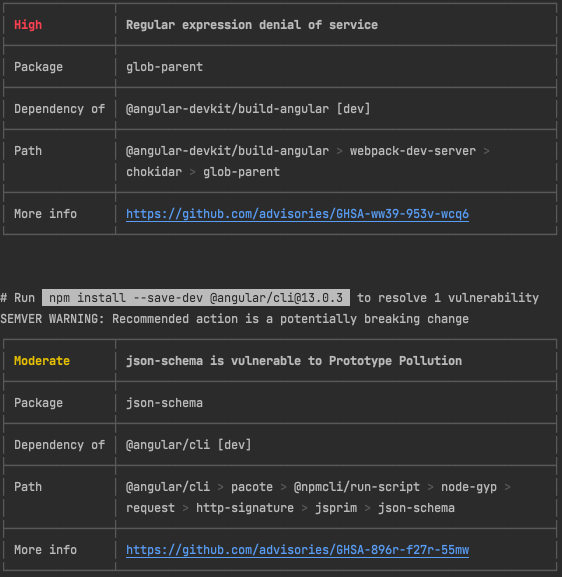
\includegraphics[width=10cm]{gfx/Screenshot NPM audit}
    \caption{Screenshot NPM audit result}
    \label{fig:npmauditresult}
\end{figure}


\subsection{SBT}\label{subsec:sbt}
Voor het analyseren van sbt projecten zijn meerdere manier. Veelal zijn dit checks die in bestaande CI-CD pipeline van bijv. GitLab, GitHub(CircleCI) worden betrokken. Een voorbeeld hiervan is een tool dat gebruik maakt van Gemnasium als analyse tool. Echter is het overhevelen van de pipeline naar Gitlab op dit moment geen optie gezien er een requirement bestaat dat de huidige pipeline moet blijven bestaan met minimale aanpassingen. De volgende optie zou zijn om een plug-in voor Jenkins te gebruiken, welke bestaat, echter is hier het probleem dat deze voor adoptie is aangeboden en er dus de kans bestaat dat de support en ontwikkeling stil komt te liggen. Deze zijn geen optie voor EagleScience omdat dit zou betekenen dat de huidige pipeline zou moeten verhuizen van de bestaande Jenkins naar een pipline aangeboden door GitLab. Welke we al gebruiken als Repository voor de geschreven code. Om toch gebruik te kunnen maken van Jenkins zou de eerst volgende optie zijn om gebruik te maken van een plugin die de check uitvoerd. Er bestaat de OWASP-dependency-check plug die analyseert of er kwetsbaarheden bestaan in een project er zijn Een voordeel zou kunnen zijn dat er quality gates toegevoegd kunnen worden aan de plugin zodat deze de build kan stoppen op het moment dat er kwetsbaarheden gevonden zijn die boven een theshold liggen. Daarnaast zijn er twee nadelen 1: De plugin wordt op het moment van schrijven ter adoptie aangeboden op de Jenkins plugins pagina. En de output die het genereerd is een XML-format. En gezien JSON makkelijker te verwerken is richting een mongodb en het feit dat de NPM als enige optie een JSON-output geeft. Is er nog een laatste optie en dat is een plug-in in het sbt project wat in staat steld om binnen een project een analyse te doen. De voordelen zijn als eerste dat deze een JSON-output geeft. Heeft de mogelijheid om ingezette worden in een pipeline door het stellen van een CVSS score theshold dat de build doet falen op hetm moment dat deze waarde wordt overschreven. (dan moet de SBT plugin wel aangeroepen worden binnen de pipeline). De sbt plugin geeft ooutpu in veschillende formats en niet onbelangrijk JSON waarmee het potentieel makkelijk te integreren is met de resultaten die uit de NPM audit komen.


\section{Methoden om vanuit de Jenkins pipeline SOUP-analyse resultaten te verkrijgen}\label{sec:methoden-om-vanuit-de-jenkins-pipeline-soup-analyse-resultaten-te-verkrijgen}
Nu we methodes hebben voor het verkrijgen van SOUP-analyse resultaten. Moet er onderzocht worden wanneer we deze analyse uitvoeren. In feite zijn er in dit geval twee opties.
\begin{enumerate}
    \item Er wordt een analyse uitgevoerd als onderdeel van de buildpipeline binnen Jenkins
    \begin{itemize}
        \item voordelen:
        \begin{itemize}
            \item alles is geintegreerd in een enkele omgeving.
        \end{itemize}
        \item nadelen:
        \begin{itemize}
            \item Build tijden kunnen langer gaan duren.
            \item moet een plugin/script komen die resultaten maakt die door de module kan worden ingelezen en weergegeven.
        \end{itemize}
    \end{itemize}
    \item of er wordt informatie over de dependencies verstuurd naar een aparte module welke daar wordt geanalyseerd
    \begin{itemize}
        \item voordelen:
        \begin{itemize}
            \item Build tijden lopen niet op omdat analyse niet in de pipeline gedaan wordt.
            \item alleen de data van de dependencies dienen te worden verstuurd Rapportage wordt gedaan door de module.
            \item
        \end{itemize}
        \item nadelen:
        \begin{itemize}
            \item resultaten zijn later beschikbaar dan de deploy gedaan is.
            \item
        \end{itemize}
    \end{itemize}
\end{enumerate}


\section{uitkomst bespreking donderdag 04-11-2021 met wessel en basbre}\label{sec:uitkomst-bespreking-donderdag-04-11-2021-met-wessel-en-basbre}

voorgestelde manier is het brengen van dependency gegevens naar een tijdelijke build waar analyse op gedaan wordt. dus: 1: dependencsies van zowel sbt, npm als docker verzamelen en deze samen met meta data over het project te sturen naar de api  2: die vervolgens een "dummy" project opzet met deze dependencies en daar een analyse op doet en deze vervolgens verwijderd. 3: De analyse wordt ingelezen en in een database gezet en als deze is gelukt wordt de "dummy" verwijderd.

Een andere manier is de hash van het commit te versturen op basis van deze hash een project aan te maken, builden en vervolgens een analyse op los te laten door de tools.

Beide hebben voor en nadelen:

\subsection{dependency gegevens versturen: [VOORKEUR vanuit basbre]}\label{subsec:dependency-gegevens-versturen:-[voorkeur-vanuit-basbre]}
\textbf{voordelen:}
versie gegevens van de gebouwde deploy geeft een veilige aanname van de gebruikte versies in een project.
\textbf{nadelen:}
er moet een tool komen die de gegevens uit de dependency declaraties haalt en deze in een schema (JSON) vorm post naar de API\@.

\subsection{hash versturen}\label{subsec:hash-versturen}
\textbf{voordelen:}
Alleen een hash meesturen naar de API is makkelijker te doen dan een volledige JSON opbouwen vergeleken met optie 1.
\textbf{nadelen:}
Niet geheel zeker welke versies er zijn gebouwd.??
